\section{General Pupropose Processors}

General Purpose Processors (GPPs) are characterized by a generic architecture that is applicable across a wide range of fields. 
They are commonly found in PCs and Personal Digital Assistants (PDAs), and for embedded systems, they are suitable for low-end applications where energy efficiency and performance are not critical, and the application nature is quite heterogeneous.
GPPs handle tasks such as controlling and managing slow interfaces with sensors and enabling interactivity through graphical user interfaces (GUIs).
GPPs can be categorized into two main architectural styles:
\begin{itemize} 
    \item \textit{Complex Instruction Set Computer} (CISC): features a large number of complex instructions. 
    \item \textit{Reduced Instruction Set Computer} (RISC): utilizes a smaller set of simple instructions. 
\end{itemize}

\subsection{Complex Instruction Set Computer} 
CISC architectures aim to allow each arithmetic or logic operation to access data and write results using any available addressing mode. 
They feature a fully orthogonal architecture and instruction set. 
However, in practice, the number of combinations of operations and addressing modes is often limited, typically with one operand referencing memory and the other being a register that acts as both source and destination.
Despite the complexity, CISC instructions are encoded in variable-length formats, which necessitates more complex fetch and decode units and a higher speed for memory access.

The Arithmetic Logic Unit (ALU) implements various basic operations such as addition, subtraction, multiplication, division, logic operations, shifting, and comparisons. 
Some architectures even support vector instructions, enabling operations on multiple registers simultaneously, indicative of a Single Instruction Multiple Data (SIMD) architecture. 
The diversity in addressing modes and arithmetic/logical operations requires a complex data path that is challenging to optimize for speed.
To enhance throughput, CISC processors often employ intricate pipelining techniques (e.g., up to 23 stages), which can be challenging to manage. 
Additionally, they may alter the order of execution for assembly instructions without changing the program's semantics. 
This complexity makes it difficult for compilers to predict instruction execution status, potentially leading to suboptimal instruction decoding. 
Modern CISC processors integrate hardware units that dynamically reschedule instructions, enabling out-of-order execution.

Although CISC architectures provide impressive performance, the focus on energy efficiency and cost has gradually shifted toward other architectures.

\subsection{Reduced Instruction Set Computer}
RISC architectures simplify instruction sets, utilizing a limited number of straightforward instructions. 
By the late 1980s, the declining prices of DRAMs and the increasing scale of integration allowed for more complex architectures on a single chip. 
CISC operations could be decomposed into multiple RISC instructions, streamlining architecture.

The primary advantages of RISC architectures include a simple instruction set and straightforward architecture, which simplify instruction decoding. 
RISC instructions typically have fixed lengths, facilitating balanced pipeline stages and higher clock speeds. 
Execution units, such as the ALU and Branch Processing Unit (BPU), benefit from simpler instructions, allowing RISC architectures to operate predominantly on registers, thus improving speed and predictability.

RISC employs a load/store architecture for input/output operations, which involves preloading data and writing results back to memory. 
While the limited number of addressing modes can aid performance, effective use of memory hierarchy is crucial for minimizing data access time.

When comparing RISC and CISC using the same high-level source code, RISC generally requires a higher number of instructions. 
RISC architectures do not have hardware mechanisms to resolve pipeline conflicts, but their predictable execution allows compilers to generate efficient code. 
Furthermore, RISC architectures typically exhibit lower power consumption due to their inherent simplicity compared to CISC architectures.

\subsection{Superscalar}
Superscalar architectures feature multiple execution units, enabling the simultaneous execution of more than one instruction per clock cycle. 
This parallelism enhances throughput but also increases the complexity of control logic, impacting clock speed and power consumption. 
In these architectures, the microprocessor dynamically schedules instructions, relieving the compiler from managing code organization for specific hardware structures. 
However, a significant portion of the processor's resources is dedicated to implementing complex scheduling mechanisms and maintaining consistency.

\subsection{Complex Instruction Set Computer and Reduced Instruction Set Computer}
Some architectures combine out-of-order execution with superscalarity while maintaining compatibility with legacy code. 
The x86 instruction set serves as the de facto standard for CISC, where each instruction is decomposed into a series of simpler instructions that can be executed by an efficient core. 
This approach incurs additional hardware costs but merges the advantages of backward compatibility with the high performance achievable through a RISC core.

\subsection{Very Long Instruction Word}
To address the challenges associated with hardware scheduling complexity, Intel developed a class of processors known as EPIC (Explicitly Parallel Instruction Computing) or VLIW (Very Long Instruction Word). 
VLIW supports explicit parallelism, allowing multiple instructions to be executed simultaneously under program control. 
A VLIW instruction consolidates multiple elementary instructions, typically of RISC nature, into a single wide word with a fixed structure.

Once fetched from memory, the VLIW word is decoded in parallel, with individual RISC instructions dispatched to various execution units. 
This fixed structure shifts the complexity of scheduling onto the compiler, which must optimize algorithms to fit the specific architecture.

The goal of EPIC/VLIW is to transfer the burden of scheduling and code optimization to the compiler, resulting in simpler architectures, although with large sizes due to the number of execution units. 
Power consumption for VLIW architectures falls between that of simpler RISC and superscalar designs. 
Similar strategies have also been implemented in specialized architectures such as digital signal processors (DSPs) to achieve peak performance.

\subsection{Complex Instruction Set Computer and Very Long Instruction Word}
Similar to the CISC/RISC relationship, VLIW architectures aim for high performance while ensuring backward compatibility. 
CISC instructions are broken down into basic instructions that can be executed by a VLIW core, which is both simple and efficient.

\subsection{Comparison}
\begin{figure}[H]
    \centering
    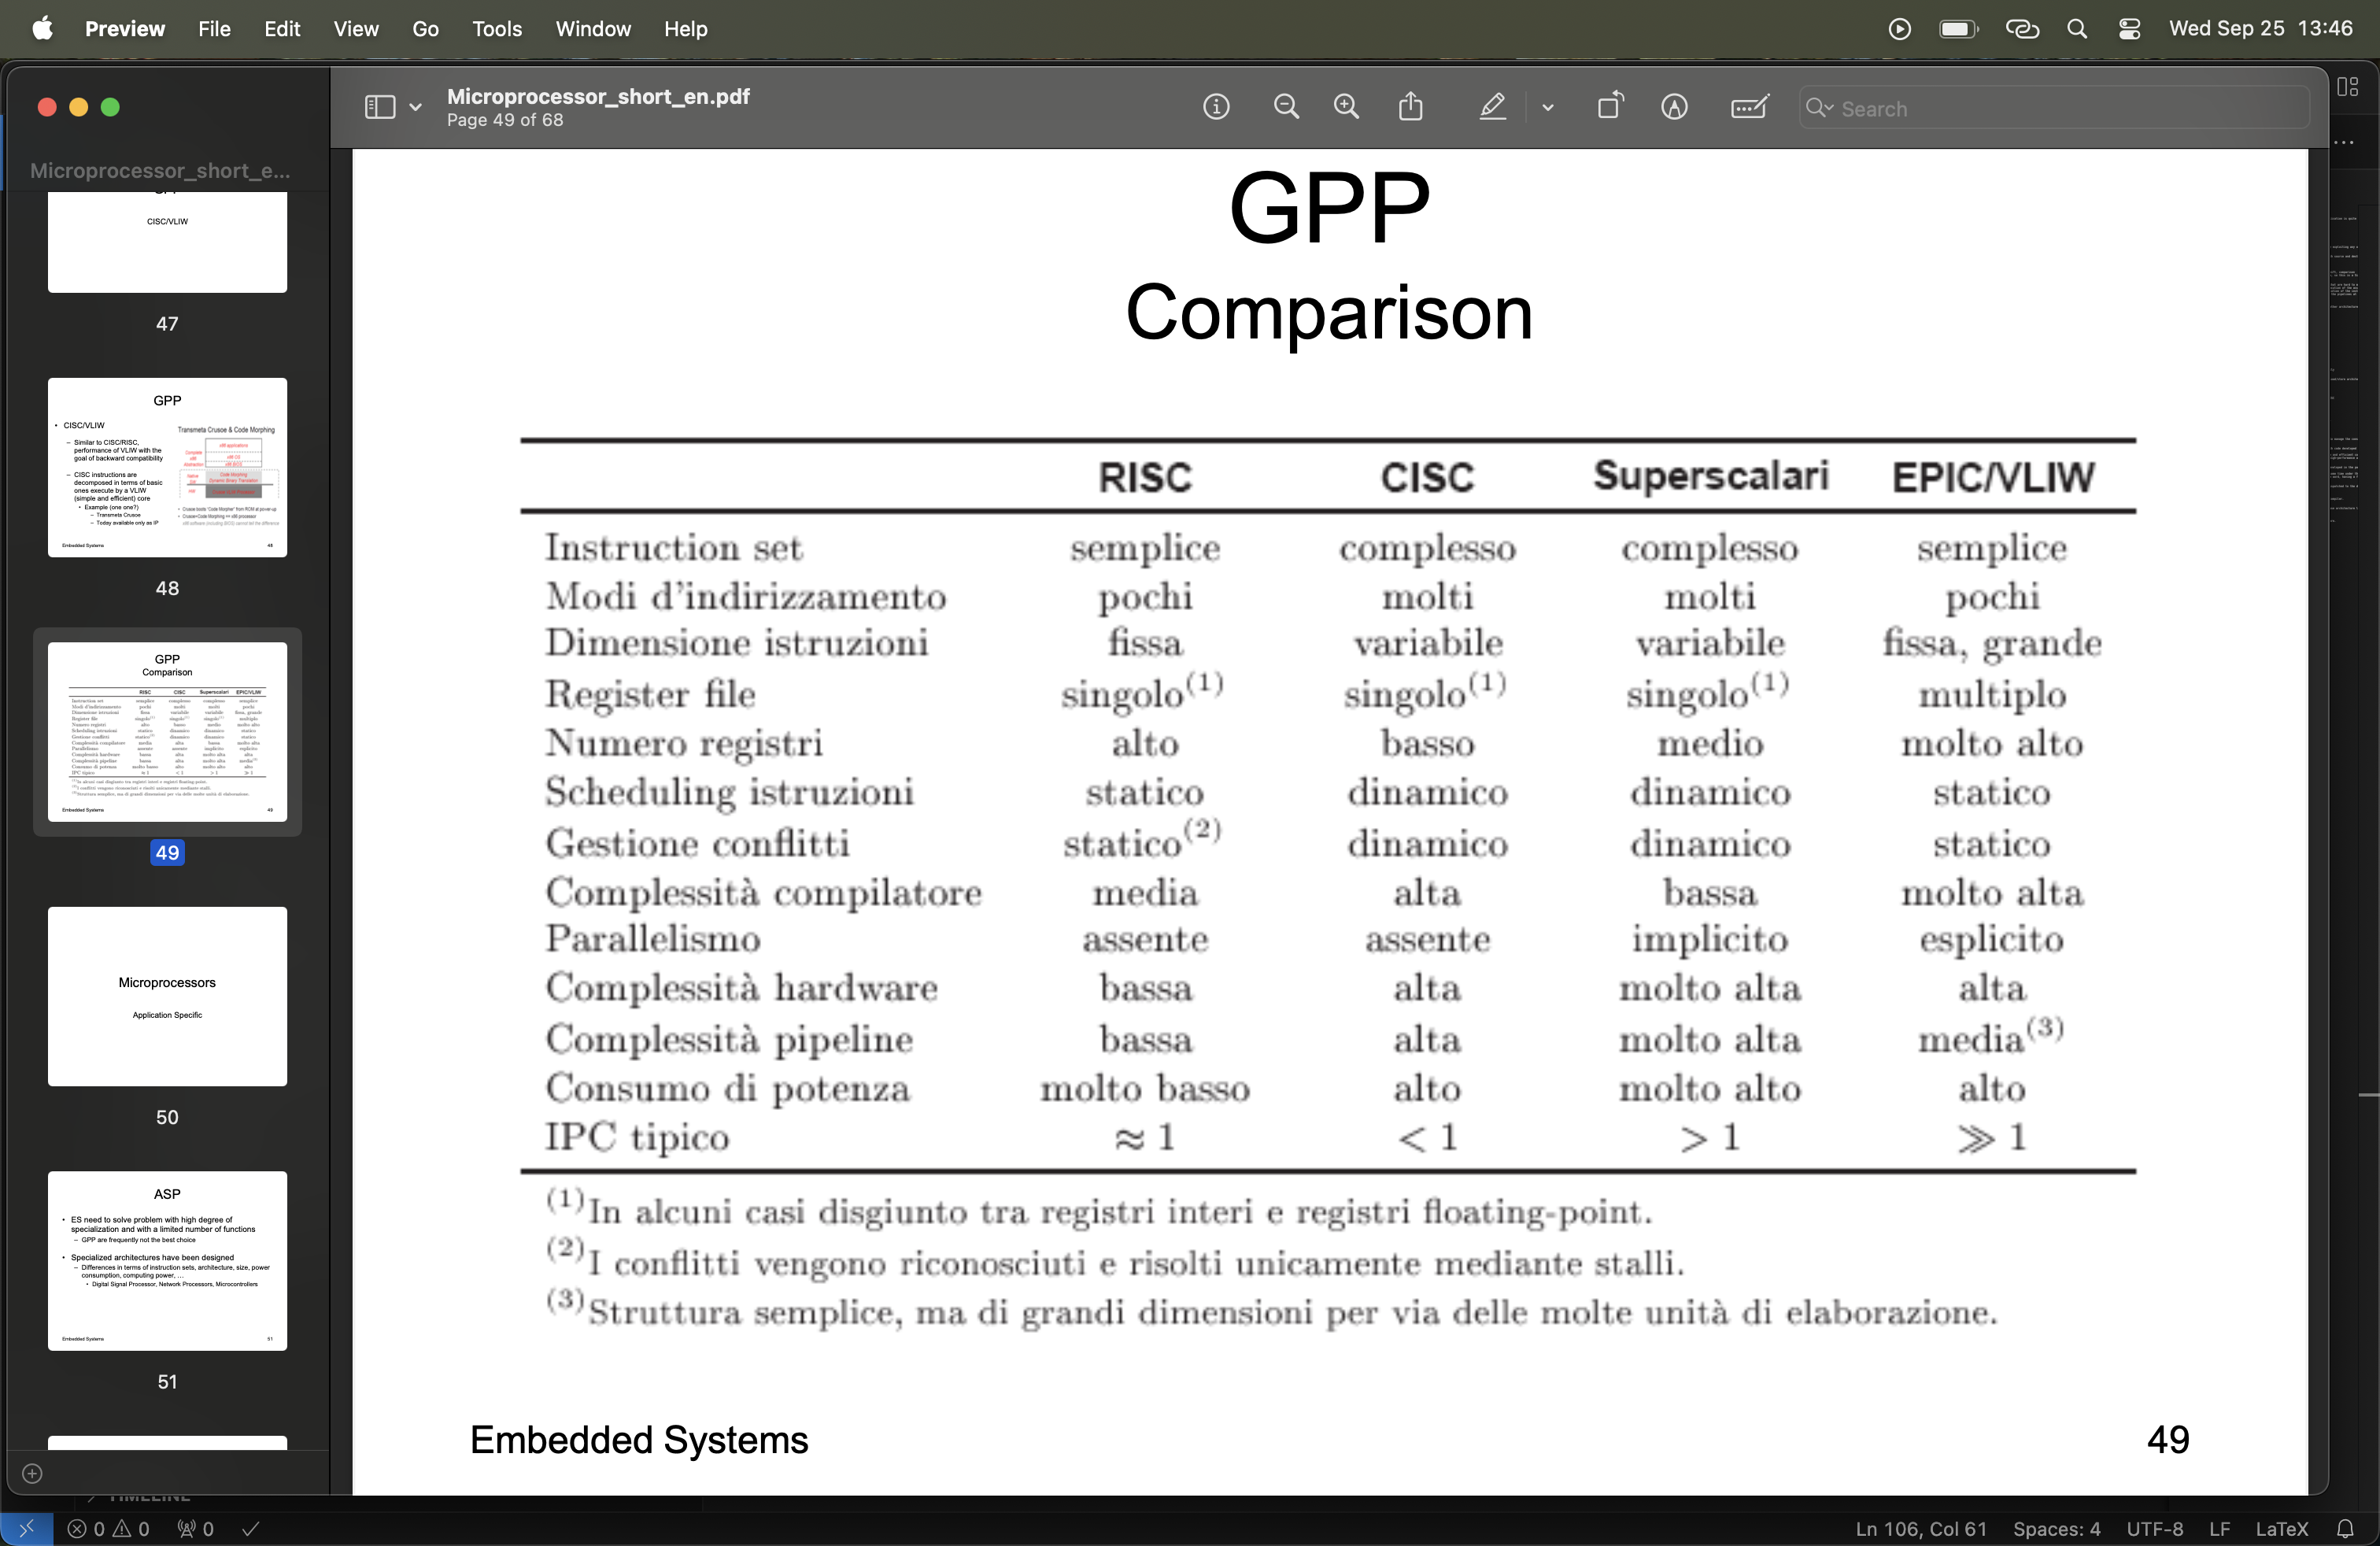
\includegraphics[width=0.75\linewidth]{images/comparison.png}
    \caption{Comp}
\end{figure}
